%==============================================================================
% MATH 110 - Section 1C Notes: Subspaces
% Linear Algebra Done Right, 4th ed. - Sheldon Axler
%==============================================================================

\documentclass[10pt, twocolumn]{article}
\usepackage[margin=0.75in, columnsep=0.3in]{geometry}

%------------------------------------------------------------------------------
% PACKAGES
%------------------------------------------------------------------------------
\usepackage{amsmath, amssymb, amsthm}
\usepackage{enumitem}
\usepackage{fancyhdr}
\usepackage{titlesec}
\usepackage{tcolorbox}
\tcbuselibrary{breakable}
\usepackage{booktabs}
\usepackage{tikz}
\usetikzlibrary{matrix, arrows.meta, positioning, calc, cd, shapes.geometric}
\usepackage{graphicx}

% TikZ style definitions for consistent diagrams (matching notes-1a, notes-1b)
\tikzset{
    vector/.style={->, >=Stealth, thick},
    axis/.style={->, thin},
    point/.style={fill, circle, inner sep=1.5pt}
}

%------------------------------------------------------------------------------
% SPACING
%------------------------------------------------------------------------------
\linespread{1.08}
\setlength{\parskip}{0.4ex plus 0.2ex minus 0.1ex}

%------------------------------------------------------------------------------
% BOX STYLES
%------------------------------------------------------------------------------
\tcbset{
    boxrule=0.8pt,
    colback=white,
    colframe=black,
    arc=0pt,
    boxsep=3pt,
    left=4pt, right=4pt, top=4pt, bottom=4pt,
    breakable
}

\newtcolorbox{result}{
    boxrule=0pt,
    colback=black!5,
    colframe=white,
    arc=0pt,
    boxsep=2pt,
    left=4pt, right=4pt, top=4pt, bottom=4pt,
    breakable
}

%------------------------------------------------------------------------------
% SECTION FORMATTING
%------------------------------------------------------------------------------
\titleformat{\section}{\large\bfseries}{\thesection.}{0.5em}{}
\titleformat{\subsection}{\normalsize\bfseries}{\thesubsection}{0.5em}{}
\titlespacing*{\section}{0pt}{1.5ex}{1ex}
\titlespacing*{\subsection}{0pt}{1ex}{0.5ex}

%------------------------------------------------------------------------------
% LIST FORMATTING
%------------------------------------------------------------------------------
\setlist{itemsep=1pt, topsep=3pt, parsep=1pt, leftmargin=1.5em}

%------------------------------------------------------------------------------
% HEADER/FOOTER
%------------------------------------------------------------------------------
\pagestyle{fancy}
\fancyhf{}
\fancyhead[L]{\small MATH 110}
\fancyhead[R]{\small Section 1C}
\fancyfoot[C]{\small\thepage}
\renewcommand{\headrulewidth}{0.4pt}

%------------------------------------------------------------------------------
% THEOREM ENVIRONMENTS
%------------------------------------------------------------------------------
\theoremstyle{definition}
\newtheorem{property}{Property}
\newtheorem{definition}{Definition}
\newtheorem{example}{Example}

\theoremstyle{plain}
\newtheorem{theorem}{Theorem}
\newtheorem{lemma}{Lemma}
\newtheorem{proposition}{Proposition}
\newtheorem{corollary}{Corollary}

%------------------------------------------------------------------------------
% CUSTOM COMMANDS
%------------------------------------------------------------------------------
% Number fields
\newcommand{\R}{\mathbb{R}}
\newcommand{\C}{\mathbb{C}}
\newcommand{\F}{\mathbb{F}}
\newcommand{\Z}{\mathbb{Z}}
\newcommand{\Q}{\mathbb{Q}}

% Matrix/space operations
\DeclareMathOperator{\rank}{rank}
\DeclareMathOperator{\nullity}{nullity}
\DeclareMathOperator{\tr}{tr}
\DeclareMathOperator{\spn}{span}
\DeclareMathOperator{\col}{col}
\DeclareMathOperator{\row}{row}
\DeclareMathOperator{\nul}{null}
\DeclareMathOperator{\range}{range}
\DeclareMathOperator{\im}{im}

% Inner products and norms
\newcommand{\inner}[2]{\langle #1, #2 \rangle}
\newcommand{\norm}[1]{\| #1 \|}
\newcommand{\proj}{\operatorname{proj}}

% Vectors and matrices
\newcommand{\vect}[1]{\mathbf{#1}}
\newcommand{\mat}[1]{\mathbf{#1}}

%==============================================================================
\begin{document}
%==============================================================================

\noindent
\begin{minipage}{\linewidth}
    \centering
    \textbf{\Large Section 1C: Subspaces} \\[0.5em]
    \hrule
\end{minipage}
\vspace{1em}

%==============================================================================
\section{Introduction to Subspaces}
%==============================================================================

Often we want to find vector spaces that ``live inside'' a larger vector space. For example, lines and planes through the origin in $\R^3$ turn out to be vector spaces in their own right. The key idea is that a subset can inherit the vector space structure from its parent.

\begin{tcolorbox}
\textbf{1.33 Definition: Subspace}

A subset $U$ of $V$ is called a \textbf{subspace} of $V$ if $U$ is also a vector space (using the same addition and scalar multiplication as on $V$).
\end{tcolorbox}

\medskip
\textbf{Key point:} A subspace uses the \textit{same} operations as the parent space. We don't invent new addition or scalar multiplication---we just restrict to a subset.

\smallskip
\begin{center}
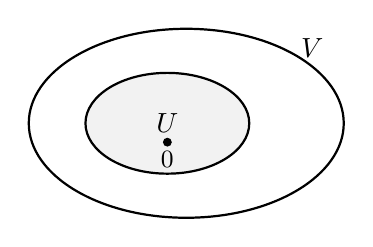
\begin{tikzpicture}[scale=0.8]
    % Outer ellipse V
    \draw[thick] (0,0) ellipse (2.5cm and 1.5cm);
    \node at (2.0,1.2) {$V$};
    % Inner ellipse U (subspace)
    \draw[thick, fill=black!5] (-0.3,0) ellipse (1.3cm and 0.8cm);
    \node at (-0.3,0) {$U$};
    % Zero vector
    \fill (-0.3,-0.3) circle (2pt) node[below] {\small$0$};
\end{tikzpicture}

\small\textit{A subspace $U$ sits inside $V$ and contains the origin.}
\end{center}
\smallskip

\textbf{Note:} The additive identity of a subspace must be the same as the additive identity of the larger space. If $0_U$ is the additive identity of $U$ and $0$ is the additive identity of $V$, then for any $v \in U$:
\[
    0_U = 0_U + 0 = 0 + 0_U = 0
\]
So subspaces always contain the zero vector of $V$.

\medskip

%==============================================================================
\section{The Subspace Test}
%==============================================================================

\medskip
Checking all 8 vector space axioms would be tedious. Fortunately, most axioms are inherited automatically. The following result gives us a simpler test.

\begin{tcolorbox}
\textbf{1.34 Conditions for a Subspace}

A subset $U$ of $V$ is a subspace of $V$ if and only if $U$ satisfies the following three conditions:

\textbf{\textcolor{blue}{additive identity:}}
\[
    0 \in U
\]

\smallskip
\textbf{\textcolor{blue}{closed under addition:}}
\[
    u, w \in U \implies u + w \in U
\]

\smallskip
\textbf{\textcolor{blue}{closed under scalar multiplication:}}
\[
    a \in \F \text{ and } u \in U \implies au \in U
\]
\end{tcolorbox}

\textbf{Proof:}

\medskip
$(\Rightarrow)$ \textit{Subspace} $\implies$ \textit{three conditions.} \textbf{(Easy direction.)}

If $U$ is a subspace, it is already a vector space. So it automatically has a zero vector, is closed under addition, and is closed under scalar multiplication. By uniqueness of the additive identity in $V$ (Result 1.26), the zero vector of $U$ must be $0$. So $0 \in U$.

\medskip
$(\Leftarrow)$ \textit{Three conditions} $\implies$ \textit{subspace.} \textbf{(Important direction.)}

Suppose $U$ satisfies the three conditions. We verify every vector space axiom:

\begin{itemize}
    \item \textbf{\textcolor{blue}{Step 1: Additive identity.}} $0 \in U$ by assumption.

    \smallskip
    \item \textbf{\textcolor{blue}{Step 2: Closure under addition.}} Closure under addition means that if $u, w \in U$, then $u + w \in U$. Addition stays inside $U$.

    \smallskip
    \item \textbf{\textcolor{blue}{Step 3: Closure under scalar multiplication.}} Closure under scalar multiplication means that if $a \in \F$ and $u \in U$, then $au \in U$. Scalar multiplication stays inside $U$.

    \smallskip
    \item \textbf{\textcolor{blue}{Step 4: Additive inverses.}} For any $u \in U$, we need $-u \in U$. Observe that
    \[
        -u = (-1)u.
    \]
    Since $-1 \in \F$ and $U$ is closed under scalar multiplication, $(-1)u \in U$. So additive inverses exist in $U$.

    \smallskip
    \item \textbf{\textcolor{blue}{Step 5: Remaining axioms.}} Commutativity, associativity, distributivity, and $1u = u$ are properties of \emph{elements}, not of the set. Since $U \subseteq V$, every element of $U$ is an element of $V$, and these equations already hold in $V$. So they hold in $U$ automatically.
\end{itemize}

All vector space axioms hold in $U$, so $U$ is a subspace of $V$. \hfill $\square$

\medskip
\begin{result}
\textbf{Big picture:} This proof explains why the Subspace Test works. It reduces checking ${\sim}8$ vector space axioms down to just 3 simple checks: zero, closed under $+$, closed under scalar $\times$. That is the test you will use constantly in Math 110.

\textbf{Why not reduce further?} The ${\sim}5$ axioms we skip (commutativity, associativity, distributivity, etc.) are \textbf{equations about elements}. If $u, w \in U \subseteq V$, then $u + w = w + u$ is already true because it is true in $V$. You cannot ``break'' commutativity by restricting to a subset. These are \emph{element properties}, and they are inherited automatically.

The 3 checks we keep are different --- they ask whether the \textbf{output} of an operation lands back in $U$. That is a property of the \emph{set}, and $V$ cannot guarantee it for you:
\begin{itemize}
    \item \textbf{Zero vector:} Without $0 \in U$, the set could be empty (and the empty set is not a vector space). This is the existence check.
    \item \textbf{Closed under $+$:} $V$ guarantees $u + w$ exists \emph{somewhere} in $V$, but not that it stays in $U$. For example, $U = \{(1,0),\, (0,1)\} \subset \R^2$ has $(1,0) + (0,1) = (1,1) \notin U$.
    \item \textbf{Closed under scalar $\times$:} Similarly, $\lambda u$ exists in $V$ but might leave $U$. For example, $U = \{(1,0)\}$ has $2 \cdot (1,0) = (2,0) \notin U$.
\end{itemize}

\begin{center}\textit{The fundamental distinction: element properties are inherited; set properties are not.}\end{center}
\end{result}

\begin{result}
\textbf{Alternative condition:} Instead of checking $0 \in U$, you can check that $U$ is \textbf{nonempty}. Here's why:

If $U \neq \emptyset$, pick any $u \in U$. By closure under scalar multiplication:
\[
    0 \cdot u = 0 \in U
\]

So ``$U$ is nonempty'' $\Leftrightarrow$ ``$0 \in U$'' when the other conditions hold.
\end{result}

\begin{tcolorbox}[colframe=black!50]
\textbf{Worked Example: Is $U = \{(x, 2x) : x \in \R\}$ a subspace of $\R^2$?}

\medskip
\textit{Geometrically, $U$ is the line $y = 2x$, which passes through the origin.}

\medskip
\textbf{\textcolor{blue}{Check the three conditions:}}
\begin{enumerate}
    \item \textbf{\textcolor{blue}{Zero vector:}} Setting $x = 0$ gives $(0, 0) \in U$. \checkmark
    \item \textbf{\textcolor{blue}{Closed under addition:}} Take $(a, 2a), (b, 2b) \in U$. Then
    \[
        (a, 2a) + (b, 2b) = (a + b,\; 2a + 2b) = \underbrace{(a + b,\; 2(a + b))}_{\text{has the form } (x,\, 2x)} \in U. \quad \checkmark
    \]
    \item \textbf{\textcolor{blue}{Closed under scalar multiplication:}} Take $\lambda \in \R$ and $(a, 2a) \in U$. Then
    \[
        \lambda (a, 2a) = (\lambda a,\; 2\lambda a) = \underbrace{(\lambda a,\; 2(\lambda a))}_{\text{has the form } (x,\, 2x)} \in U. \quad \checkmark
    \]
\end{enumerate}

\textbf{\textcolor{blue}{Conclusion:}} $U$ is a subspace of $\R^2$.

\medskip
\textit{Remark:} Any line through the origin in $\R^2$ is a subspace. A line that does \emph{not} pass through the origin, such as $\{(x, 2x + 1) : x \in \R\}$, fails the zero vector condition and is \emph{not} a subspace.
\end{tcolorbox}

\newpage
%==============================================================================
\section{Examples of Subspaces}
%==============================================================================

\begin{tcolorbox}[colframe=black!50]
\textbf{1.35(a) Example: $\{(x_1, x_2, x_3, x_4) \in \F^4 : x_3 = 5x_4 + b\}$}

Let $b \in \F$ and define
\[
    U = \{(x_1, x_2, x_3, x_4) \in \F^4 : x_3 = 5x_4 + b\}.
\]
We will show that $U$ is a subspace of $\F^4$ if and only if $b = 0$.

\smallskip
\textbf{\textcolor{blue}{Step 0:}} $U \subseteq V$: Every element of $U$ is a $4$-tuple in $\F^4$, so $U \subseteq \F^4$. By the subspace test, $U$ is a subspace of $\F^4$ if and only if it contains the zero vector and is closed under addition and scalar multiplication.

\bigskip
\textbf{\textcolor{blue}{Direction 1 ($b \neq 0$): $U$ is not a subspace.}}

\smallskip
\textbf{\textcolor{blue}{Step 1:}} Check the zero vector. The zero vector in $\F^4$ is $\mathbf{0} = (0, 0, 0, 0)$. We need $x_3 = 5x_4 + b$, so plugging in gives
\[
    0 = 5 \cdot 0 + b = b.
\]
Thus $\mathbf{0} \in U$ if and only if $b = 0$. If $b \neq 0$, then $\mathbf{0} \notin U$, so $U$ is \emph{not} a subspace. $\boldsymbol{\times}$

\bigskip
\textbf{\textcolor{blue}{Direction 2 ($b = 0$): $U$ is a subspace.}}

\smallskip
Now $U = \{(x_1, x_2, x_3, x_4) \in \F^4 : x_3 = 5x_4\}$. We verify the three subspace conditions.

\smallskip
\textbf{\textcolor{blue}{Step 2:}} Contains $\mathbf{0}$. The vector $(0, 0, 0, 0)$ satisfies $0 = 5 \cdot 0$, so $\mathbf{0} \in U$. \checkmark

\smallskip
\textbf{\textcolor{blue}{Step 3:}} Closed under addition. Let $u = (x_1, x_2, x_3, x_4)$ and $w = (y_1, y_2, y_3, y_4)$ be elements of $U$, so $x_3 = 5x_4$ and $y_3 = 5y_4$. Then
\[
    u + w = (x_1 + y_1,\; x_2 + y_2,\; x_3 + y_3,\; x_4 + y_4).
\]
The third component of $u + w$ is $x_3 + y_3 = 5x_4 + 5y_4 = 5(x_4 + y_4)$, which equals $5$ times the fourth component. Hence $u + w \in U$. \checkmark

\smallskip
\textbf{\textcolor{blue}{Step 4:}} Closed under scalar multiplication. Let $a \in \F$ and $u = (x_1, x_2, x_3, x_4) \in U$, so $x_3 = 5x_4$. Then
\[
    au = (ax_1,\; ax_2,\; ax_3,\; ax_4).
\]
The third component of $au$ is $ax_3 = a(5x_4) = 5(ax_4)$, which equals $5$ times the fourth component. Hence $au \in U$. \checkmark

\smallskip
\textbf{\textcolor{blue}{Conclusion:}} All three conditions are satisfied when $b = 0$, so $U$ is a subspace of $\F^4$ if and only if $b = 0$.
\end{tcolorbox}

\begin{result}
\textbf{Lesson:} Subspaces must pass through the origin. A constraint like $x_3 = 5x_4 + b$ with $b \neq 0$ defines an ``affine subspace'' (a shifted subspace), not a true subspace.
\end{result}

\medskip
\begin{tcolorbox}[colframe=black!50]
\textbf{1.35(b) Example: Continuous Functions}

Let $V = \R^{[0,1]}$ be the vector space of all real-valued functions on $[0,1]$, and let
\[
    U = C([0,1]) = \{\text{continuous real-valued functions on } [0,1]\}.
\]
We will show that $U$ is a subspace of $V$.

\smallskip
\textbf{\textcolor{blue}{Step 0:}} Every continuous function $f \colon [0,1] \to \R$ is certainly a function $[0,1] \to \R$, so $U \subseteq V$. By the subspace test, it suffices to verify three conditions.

\smallskip
\textbf{\textcolor{blue}{Step 1:}} Check the zero vector. In $V = \R^{[0,1]}$, the zero vector is the \emph{zero function}:
\[
    f_0(x) = 0 \quad \text{for all } x \in [0,1].
\]
This function is continuous on $[0,1]$, so $f_0 \in U$. \checkmark

\smallskip
\textbf{\textcolor{blue}{Step 2:}} Check closure under addition. Let $f, g \in U$, so $f$ and $g$ are continuous on $[0,1]$. Their sum $f + g$ is defined by
\[
    (f + g)(x) = f(x) + g(x).
\]
By a standard fact from calculus, the sum of continuous functions is continuous. So $f + g$ is continuous on $[0,1]$, hence $f + g \in U$. \checkmark

\smallskip
\textbf{\textcolor{blue}{Step 3:}} Check closure under scalar multiplication. Let $a \in \R$ and $f \in U$, so $f$ is continuous on $[0,1]$. The scalar multiple $af$ is defined by
\[
    (af)(x) = a \cdot f(x).
\]
By a standard fact from calculus, a constant times a continuous function is continuous. So $af$ is continuous on $[0,1]$, hence $af \in U$. \checkmark

\smallskip
\textbf{\textcolor{blue}{Conclusion:}} Since $U$ contains the zero function and is closed under addition and scalar multiplication, $C([0,1])$ is a subspace of $\R^{[0,1]}$.
\end{tcolorbox}

\medskip
\begin{tcolorbox}[colframe=black!50]
\textbf{1.35(c) Example: Differentiable Functions}

The set of differentiable real-valued functions on $\R$ is a subspace of $\R^\R$.

\smallskip
\textbf{\textcolor{blue}{Step 0:}} Identify the spaces. Let $V = \R^\R$ be the vector space of all functions $\R \to \R$, and let
\[
    U = \{f \in \R^\R : f \text{ is differentiable on } \R\}.
\]
Every differentiable function $\R \to \R$ is certainly a function $\R \to \R$, so $U \subseteq V$. By the subspace test, it suffices to verify three conditions.

\smallskip
\textbf{\textcolor{blue}{Step 1:}} Check the zero vector. In $V = \R^\R$, the zero vector is the \emph{zero function}:
\[
    f_0(x) = 0 \quad \text{for all } x \in \R.
\]
This function is differentiable everywhere, with $f_0'(x) = 0$ for all $x \in \R$. So $f_0 \in U$. \checkmark

\smallskip
\textbf{\textcolor{blue}{Step 2:}} Check closure under addition. Let $f, g \in U$, so $f$ and $g$ are differentiable on $\R$. Their sum $f + g$ is defined by
\[
    (f + g)(x) = f(x) + g(x).
\]
By the \emph{sum rule} from calculus, $(f + g)'(x) = f'(x) + g'(x)$. Since both $f'$ and $g'$ exist for all $x \in \R$, the derivative of $f + g$ exists everywhere. So $f + g$ is differentiable, hence $f + g \in U$. \checkmark

\smallskip
\textbf{\textcolor{blue}{Step 3:}} Check closure under scalar multiplication. Let $a \in \R$ and $f \in U$, so $f$ is differentiable on $\R$. The scalar multiple $af$ is defined by
\[
    (af)(x) = a \cdot f(x).
\]
By the \emph{constant multiple rule} from calculus, $(af)'(x) = a \cdot f'(x)$. Since $f'$ exists for all $x \in \R$, the derivative of $af$ exists everywhere. So $af$ is differentiable, hence $af \in U$. \checkmark

\smallskip
\textbf{\textcolor{blue}{Conclusion:}} Since $U$ contains the zero function and is closed under addition and scalar multiplication, the set of differentiable functions is a subspace of $\R^\R$.

\smallskip
\textbf{\textcolor{blue}{Chain of subspaces:}} Each level of smoothness gives a subspace of the next:
\[
    \{\text{polynomials}\} \subseteq C^\infty \subseteq \cdots \subseteq C^1 \subseteq C^0 \subseteq \R^\R
\]
where $C^0$ = continuous functions, $C^1$ = once-differentiable, \ldots, $C^\infty$ = infinitely differentiable (smooth). Each inclusion holds because every differentiable function is continuous, every twice-differentiable function is differentiable, and so on.
\end{tcolorbox}

\begin{result}
\textbf{Big-picture reason:} Differentiability is preserved under linear combinations: if $f$ and $g$ are differentiable and $a, b \in \R$, then $af + bg$ is differentiable. Any property preserved under linear combinations gives a subspace.
\end{result}

\medskip
\begin{tcolorbox}[colframe=black!50]
\textbf{1.35(d) Example: $\{f \in \R^{(0,3)} : f \text{ differentiable and } f'(2) = b\}$}

Let $b \in \R$ and define
\[
    U_b = \{f \in \R^{(0,3)} : f \text{ is differentiable on } (0,3) \text{ and } f'(2) = b\}.
\]
Let $V = \R^{(0,3)}$ be the vector space of all functions $(0,3) \to \R$. We will show that $U_b$ is a subspace of $V$ if and only if $b = 0$.

\smallskip
\textbf{\textcolor{blue}{Step 0:}} $U_b \subseteq V$: Every differentiable function $(0,3) \to \R$ is certainly a function $(0,3) \to \R$, so $U_b \subseteq V$.

\bigskip
\textbf{\textcolor{blue}{Direction 1 ($b \neq 0$): $U_b$ is not a subspace.}}

\smallskip
\textbf{\textcolor{blue}{Step 1:}} Check the zero vector. In $V = \R^{(0,3)}$, the zero vector is the zero function $f_0(x) = 0$ for all $x \in (0,3)$. Its derivative is $f_0'(x) = 0$ for all $x$, so $f_0'(2) = 0$. For $f_0 \in U_b$ we need $f_0'(2) = b$, i.e.\ $0 = b$. If $b \neq 0$, then $f_0 \notin U_b$, so $U_b$ does not contain the zero vector and is \emph{not} a subspace. $\boldsymbol{\times}$

\bigskip
\textbf{\textcolor{blue}{Direction 2 ($b = 0$): $U_0$ is a subspace.}}

\smallskip
Now $U_0 = \{f \in \R^{(0,3)} : f \text{ is differentiable on } (0,3) \text{ and } f'(2) = 0\}$. We verify the three subspace conditions.

\smallskip
\textbf{\textcolor{blue}{Step 2:}} Contains the zero vector. The zero function $f_0(x) = 0$ has $f_0'(2) = 0$, so $f_0 \in U_0$. \checkmark

\smallskip
\textbf{\textcolor{blue}{Step 3:}} Closed under addition. Let $f, g \in U_0$, so $f$ and $g$ are differentiable on $(0,3)$ with $f'(2) = 0$ and $g'(2) = 0$. By the \emph{sum rule} from calculus,
\[
    (f + g)'(2) = f'(2) + g'(2) = 0 + 0 = 0.
\]
So $f + g$ is differentiable on $(0,3)$ with $(f+g)'(2) = 0$, hence $f + g \in U_0$. \checkmark

\smallskip
\textbf{\textcolor{blue}{Step 4:}} Closed under scalar multiplication. Let $a \in \R$ and $f \in U_0$, so $f$ is differentiable on $(0,3)$ with $f'(2) = 0$. By the \emph{constant multiple rule} from calculus,
\[
    (af)'(2) = a \cdot f'(2) = a \cdot 0 = 0.
\]
So $af$ is differentiable on $(0,3)$ with $(af)'(2) = 0$, hence $af \in U_0$. \checkmark

\smallskip
\textbf{\textcolor{blue}{Conclusion:}} All three conditions are satisfied when $b = 0$, so $U_0$ is a subspace of $V$. Combined with Direction~1: $U_b$ is a subspace of $\R^{(0,3)}$ if and only if $b = 0$.
\end{tcolorbox}

\begin{result}
\textbf{Trick insight:} The condition $f'(2) = b$ is a \emph{linear} condition on the function $f$ only when $b = 0$; when $b \neq 0$ it is an affine shift, so the zero function fails. This is the function-space analogue of Example~(a), where $x_3 = 5x_4 + b$ is a subspace condition only when $b = 0$.
\end{result}

\begin{result}
\textbf{Proof tricks used:}
\begin{itemize}[leftmargin=*, itemsep=2pt]
    \item \textbf{``For which $b$?'' $\Rightarrow$ iff proof.} When the problem asks ``for which values of a parameter is this a subspace?'', structure the proof as two directions: one showing failure, the other showing all three conditions hold.
    \item \textbf{Zero vector test kills $b \neq 0$ immediately.} Before checking closure properties, always test whether the zero vector belongs to the set. If it doesn't, you're done --- the set is not a subspace. This is the fastest way to rule out non-subspaces.
    \item \textbf{Derivative rules do the heavy lifting.} The \emph{sum rule} $(f+g)' = f' + g'$ gives closure under addition; the \emph{constant multiple rule} $(af)' = a \cdot f'$ gives closure under scalar multiplication. In function-space subspace proofs, calculus rules translate directly into subspace conditions.
    \item \textbf{Evaluating at a point preserves linearity.} The key computation $f'(2) + g'(2) = 0 + 0 = 0$ works because differentiation is linear \emph{and} evaluation at a point is linear. The condition ``$f'(2) = 0$'' composes two linear operations: differentiate, then evaluate at $2$.
    \item \textbf{Homogeneous vs.\ non-homogeneous.} A condition of the form $L(f) = 0$ (where $L$ is a linear operation) always gives a subspace. A condition $L(f) = b$ with $b \neq 0$ never does, because $L(f_0) = L(0) = 0 \neq b$. This pattern appears whenever a parameter $b$ shifts the constraint away from zero.
\end{itemize}
\end{result}

\medskip
\begin{tcolorbox}[colframe=black!50]
\textbf{1.35(e) Example: Sequences Converging to 0}

Let $V = \C^\infty$ be the vector space of all complex sequences
\[
    (a_1, a_2, a_3, \ldots), \quad a_n \in \C
\]
with addition and scalar multiplication defined term-by-term. Let
\[
    U = \{(a_n) \in \C^\infty : \lim_{n \to \infty} a_n = 0\}.
\]
\textbf{\textcolor{blue}{Claim:}} $U$ is a subspace of $V$.

\smallskip
\textbf{\textcolor{blue}{Step 0:}} $U \subseteq V$: Every sequence with limit $0$ is still a complex sequence, so $U \subseteq \C^\infty$.

\smallskip
\textbf{\textcolor{blue}{Step 1:}} Check $\mathbf{0} \in U$. The zero vector in $\C^\infty$ is the zero sequence:
\[
    \mathbf{0} = (0, 0, 0, \ldots).
\]
Its limit is $\lim_{n \to \infty} 0 = 0$, so $\mathbf{0} \in U$. \checkmark

\smallskip
\textbf{\textcolor{blue}{Step 2:}} Closed under addition. Take any $(a_n), (b_n) \in U$, so
\[
    \lim_{n \to \infty} a_n = 0, \qquad \lim_{n \to \infty} b_n = 0.
\]
Consider their sum $(a_n + b_n)$. By the limit sum law:
\[
    \lim_{n \to \infty} (a_n + b_n) = \lim_{n \to \infty} a_n + \lim_{n \to \infty} b_n = 0 + 0 = 0.
\]
So $(a_n + b_n) \in U$. \checkmark

\smallskip
\textbf{\textcolor{blue}{Step 3:}} Closed under scalar multiplication. Take $(a_n) \in U$ and $c \in \C$, so $\lim a_n = 0$. By the limit scalar law:
\[
    \lim_{n \to \infty} (c \, a_n) = c \cdot \lim_{n \to \infty} a_n = c \cdot 0 = 0.
\]
So $(c \, a_n) \in U$. \checkmark

\smallskip
\textbf{\textcolor{blue}{Conclusion:}} Since $U$ contains the zero sequence and is closed under addition and scalar multiplication, $U$ is a subspace of $\C^\infty$.
\end{tcolorbox}

\begin{result}
\textbf{Trick insight:} Anything defined by ``limit equals $0$'' tends to be a subspace because limits respect linear combinations:
\[
    \lim(c \, a_n + d \, b_n) = c \lim a_n + d \lim b_n.
\]
Compare: the set of sequences with limit $1$ is \emph{not} a subspace --- the zero sequence has limit $0 \neq 1$.
\end{result}

\begin{result}
\textbf{Pattern:} Across all these examples, constraints of the form ``something $= 0$'' (homogeneous) tend to give subspaces, because the zero vector satisfies them and the arithmetic of $0$ plays nicely with addition and scaling. Constraints of the form ``something $= b$'' with $b \neq 0$ (non-homogeneous) do \emph{not} give subspaces, because they exclude the zero vector. This pattern appears in both finite-dimensional settings (Example~(a): $x_3 = 5x_4 + b$) and function spaces (Example~(d): $f'(2) = b$).
\end{result}

\medskip
\begin{result}
\textbf{Extreme subspaces:} Every vector space $V$ has two ``trivial'' subspaces:
\begin{itemize}
    \item The \textbf{smallest subspace}: $\{0\}$ (just the zero vector)
    \item The \textbf{largest subspace}: $V$ itself
\end{itemize}

\textbf{Why the empty set is not a subspace:} $\emptyset$ fails the condition $0 \in U$. Every subspace must contain the zero vector.
\end{result}

%==============================================================================
\section{Sums of Subspaces}
%==============================================================================

Given subspaces $U_1, \ldots, U_m$ of $V$, we want to build new subspaces from them. The natural candidate---the union---usually fails.

\textbf{Why not unions?} If $U$ and $W$ are subspaces of $V$, then $U \cup W$ is \textit{usually not} a subspace. For example, in $\R^2$:
\begin{itemize}
    \item Let $U = \{(x, 0) : x \in \R\}$ (the $x$-axis)
    \item Let $W = \{(0, y) : y \in \R\}$ (the $y$-axis)
    \item Then $(1, 0) \in U$ and $(0, 1) \in W$
    \item But $(1, 0) + (0, 1) = (1, 1) \notin U \cup W$
\end{itemize}

\smallskip
\begin{center}
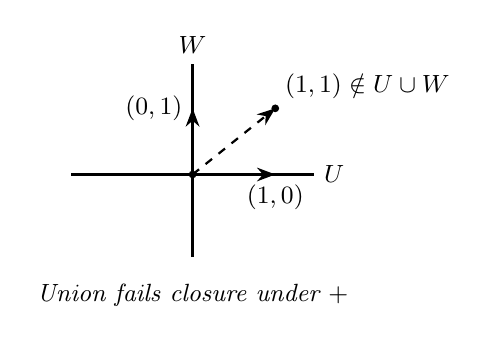
\begin{tikzpicture}[scale=0.7]
    % Axes (representing the union)
    \draw[thick] (-2.2,0) -- (2.2,0) node[right] {\small$U$};
    \draw[thick] (0,-1.5) -- (0,2) node[above] {\small$W$};
    % Origin
    \fill (0,0) circle (2pt);
    % Vectors
    \draw[vector] (0,0) -- (1.5,0) node[below] {\small$(1,0)$};
    \draw[vector] (0,0) -- (0,1.2) node[left] {\small$(0,1)$};
    % Sum vector (not in union)
    \draw[vector, dashed] (0,0) -- (1.5,1.2);
    \fill (1.5,1.2) circle (2pt) node[above right] {\small$(1,1) \notin U \cup W$};
    % Label
    \node at (0,-2.2) {\small\textit{Union fails closure under $+$}};
\end{tikzpicture}
\end{center}
\smallskip

The union is not closed under addition! We need something else.

\begin{tcolorbox}
\textbf{1.36 Definition: Sum of Subspaces}

Suppose $U_1, \ldots, U_m$ are subspaces of $V$. The \textbf{sum} of $U_1, \ldots, U_m$, denoted $U_1 + \cdots + U_m$, is the set of all possible sums of elements of $U_1, \ldots, U_m$:
\[
    U_1 + \cdots + U_m = \{u_1 + \cdots + u_m : u_j \in U_j\}
\]
\end{tcolorbox}

\begin{result}
\textbf{Notation: What does ``$\mid$'' or ``$:$'' mean?}

The definition above uses \textbf{set-builder notation}. In
\[
    U_1 + \cdots + U_m = \{u_1 + \cdots + u_m \mid u_j \in U_j\},
\]
the vertical bar ``$\mid$'' means \textbf{``such that.''} You read it as:

\smallskip
\begin{quote}
The set of all vectors of the form $u_1 + \cdots + u_m$ \textbf{such that} each $u_j \in U_j$.
\end{quote}

\smallskip
In general, $\{\text{expression} \mid \text{condition}\}$ means ``all expressions where the condition holds.'' For example,
\[
    \{x \in \R \mid x > 0\} \quad = \quad \text{all real numbers such that } x > 0.
\]

So in the sum-of-subspaces definition:
\begin{enumerate}[leftmargin=*, itemsep=1pt]
    \item Pick one vector $u_1$ from $U_1$,
    \item Pick one vector $u_2$ from $U_2$,
    \item \ldots
    \item Add them together,
    \item Collect all possible such sums.
\end{enumerate}

\smallskip
\textit{Remark:} You will also see a colon in place of the bar: $\{x \in V : \text{something about } x\}$. Both ``$\mid$'' and ``$:$'' mean the same thing --- ``such that.''
\end{result}

\medskip
\textbf{Key insight:} The sum $U_1 + \cdots + U_m$ is the \textit{smallest} subspace of $V$ containing all of $U_1, \ldots, U_m$.

\textbf{Verification that the sum is a subspace:}
\begin{itemize}
    \item $0 = 0 + \cdots + 0 \in U_1 + \cdots + U_m$ \checkmark
    \item Closed under addition: $(u_1 + \cdots + u_m) + (v_1 + \cdots + v_m) = (u_1 + v_1) + \cdots + (u_m + v_m)$, and each $u_j + v_j \in U_j$. \checkmark
    \item Closed under scalar mult: $\lambda(u_1 + \cdots + u_m) = \lambda u_1 + \cdots + \lambda u_m$, and each $\lambda u_j \in U_j$. \checkmark
\end{itemize}

\begin{tcolorbox}[colframe=black!50]
\textbf{1.37 Example: Sum of Subspaces of $\F^3$}

Let $U = \{(x, 0, 0) \in \F^3 : x \in \F\}$ (the $x$-axis).

Let $W = \{(0, y, 0) \in \F^3 : y \in \F\}$ (the $y$-axis).

Then:
\[
    U + W = \{(x, y, 0) \in \F^3 : x, y \in \F\}
\]

This is the $xy$-plane! A general element of $U + W$ is:
\[
    (x, 0, 0) + (0, y, 0) = (x, y, 0)
\]
\end{tcolorbox}

\medskip
\begin{tcolorbox}[colframe=black!50]
\textbf{1.38 Example: Sum of Subspaces of $\F^4$}

Let $U = \{(x, x, y, y) \in \F^4 : x, y \in \F\}$.

Let $W = \{(x, x, x, y) \in \F^4 : x, y \in \F\}$.

\textbf{\textcolor{blue}{Claim:}} $U + W = \{(x, x, y, z) \in \F^4 : x, y, z \in \F\}$.

\textbf{\textcolor{blue}{Proof of $\subseteq$:}} Take $u \in U$ and $w \in W$:
\begin{align*}
    u &= (a, a, b, b) \quad \text{for some } a, b \in \F \\
    w &= (c, c, c, d) \quad \text{for some } c, d \in \F \\
    u + w &= (a+c, a+c, b+c, b+d)
\end{align*}
Notice that the first two coordinates are equal. So $u + w$ has the form $(x, x, y, z)$.

\textbf{\textcolor{blue}{Proof of $\supseteq$:}} \textbf{(1.39)} Given $(x, x, y, z) \in \F^4$, we want to write it as $u + w$ with $u \in U$ and $w \in W$.

Choose:
\begin{align*}
    u &= (x, x, y, y) \in U \\
    w &= (0, 0, 0, z-y) \in W \quad \text{(since } (0, 0, 0, z-y) \text{ has form } (t, t, t, s) \text{ with } t=0)
\end{align*}

Then $u + w = (x, x, y, y) + (0, 0, 0, z-y) = (x, x, y, z)$. \checkmark
\end{tcolorbox}

%==============================================================================
\section{Sum is Smallest Containing Subspace}
%==============================================================================

\begin{tcolorbox}
\textbf{1.40 Sum of Subspaces is the Smallest Containing Subspace}

Suppose $U_1, \ldots, U_m$ are subspaces of $V$. Then $U_1 + \cdots + U_m$ is the smallest subspace of $V$ containing $U_1, \ldots, U_m$.
\end{tcolorbox}

\textbf{What ``smallest'' means:} A subspace $W$ is the smallest subspace containing $U_1, \ldots, U_m$ if:
\begin{enumerate}
    \item $U_j \subseteq W$ for all $j = 1, \ldots, m$
    \item If $S$ is any subspace containing all $U_j$, then $W \subseteq S$
\end{enumerate}

\smallskip
\textbf{Proof:}

First, we show that each $U_j \subseteq U_1 + \cdots + U_m$:

For any $u \in U_j$, we can write:
\[
    u = 0 + \cdots + 0 + u + 0 + \cdots + 0
\]
where $u$ is in the $j$-th position. Since $0 \in U_k$ for all $k \neq j$, this shows $u \in U_1 + \cdots + U_m$.

Second, we show that $U_1 + \cdots + U_m$ is contained in any subspace $S$ that contains all $U_j$:

Suppose $S$ is a subspace of $V$ containing each $U_j$. Take any element $u_1 + \cdots + u_m \in U_1 + \cdots + U_m$.

Since $u_j \in U_j \subseteq S$ for each $j$, and $S$ is closed under addition, we have:
\[
    u_1 + \cdots + u_m \in S
\]

Therefore $U_1 + \cdots + U_m \subseteq S$. \hfill $\square$

\smallskip

%==============================================================================
\section{Direct Sums}
%==============================================================================

Given a sum $U_1 + \cdots + U_m$, we know every element can be written as $u_1 + \cdots + u_m$ with $u_j \in U_j$. But can an element be written in \textit{multiple} ways? When the representation is always \textbf{unique}, the sum is called a \textbf{direct sum}.

\begin{tcolorbox}
\textbf{1.41 Definition: Direct Sum}

Suppose $U_1, \ldots, U_m$ are subspaces of $V$.
\begin{itemize}
    \item The sum $U_1 + \cdots + U_m$ is called a \textbf{direct sum} if each element of $U_1 + \cdots + U_m$ can be written in only one way as a sum $u_1 + \cdots + u_m$, where each $u_j \in U_j$.
    \item If $U_1 + \cdots + U_m$ is a direct sum, then we write $U_1 \oplus \cdots \oplus U_m$ instead of $U_1 + \cdots + U_m$.
\end{itemize}
\end{tcolorbox}

\medskip
\textbf{Notation:} The symbol $\oplus$ (``direct sum'') signals that every element has a \textit{unique} decomposition into summands from each subspace.

\smallskip
\begin{center}
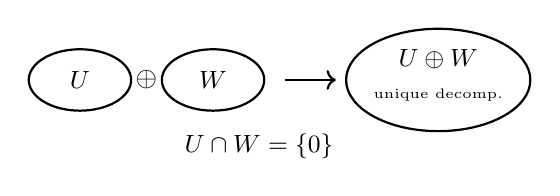
\begin{tikzpicture}[scale=0.65]
    % Left side: Direct sum
    \draw[thick] (0,0) ellipse (1cm and 0.6cm);
    \node at (0,0) {\small$U$};
    \node at (1.3,0) {$\oplus$};
    \draw[thick] (2.6,0) ellipse (1cm and 0.6cm);
    \node at (2.6,0) {\small$W$};
    % Arrow
    \draw[->, thick] (4,0) -- (5,0);
    % Right side: Result
    \draw[thick] (7,0) ellipse (1.8cm and 1cm);
    \node at (7,0.4) {\small$U \oplus W$};
    \node at (7,-0.3) {\tiny unique decomp.};
    % Condition
    \node at (3.5,-1.3) {\small$U \cap W = \{0\}$};
\end{tikzpicture}

\small\textit{Direct sum: unique decomposition when subspaces meet only at $0$.}
\end{center}
\smallskip

\begin{tcolorbox}[colframe=black!50]
\textbf{1.42 Example: $\F^3$ as a Direct Sum}

Let $U = \{(x, y, 0) \in \F^3 : x, y \in \F\}$ (the $xy$-plane).

Let $W = \{(0, 0, z) \in \F^3 : z \in \F\}$ (the $z$-axis).

\textbf{\textcolor{blue}{Claim:}} $\F^3 = U \oplus W$.

\textbf{\textcolor{blue}{Proof:}} Take any $(x, y, z) \in \F^3$. We can write:
\[
    (x, y, z) = (x, y, 0) + (0, 0, z)
\]
where $(x, y, 0) \in U$ and $(0, 0, z) \in W$. This shows $\F^3 = U + W$.

Is this decomposition unique? Suppose $(x, y, z) = (a, b, 0) + (0, 0, c)$ for some $a, b, c \in \F$.

Then $(x, y, z) = (a, b, c)$, which forces $a = x$, $b = y$, $c = z$.

So the decomposition is unique, and $\F^3 = U \oplus W$. \checkmark
\end{tcolorbox}

\medskip
\begin{tcolorbox}[colframe=black!50]
\textbf{1.43 Example: $\F^n$ as Direct Sum of Coordinate Axes}

For $j = 1, \ldots, n$, define:
\[
    U_j = \{(0, \ldots, 0, x, 0, \ldots, 0) \in \F^n : x \in \F\}
\]
where $x$ is in the $j$-th coordinate (all other coordinates are $0$).

Then:
\[
    \F^n = U_1 \oplus U_2 \oplus \cdots \oplus U_n
\]

\textbf{\textcolor{blue}{Why?}} Any $(x_1, \ldots, x_n) \in \F^n$ can be written uniquely as:
\[
    (x_1, 0, \ldots, 0) + (0, x_2, 0, \ldots, 0) + \cdots + (0, \ldots, 0, x_n)
\]

The coordinates completely determine each summand, so the decomposition is unique.
\end{tcolorbox}

%==============================================================================
\section{Testing for Direct Sums}
%==============================================================================

How can we tell if a sum is direct? The following result gives a simple test.

\begin{tcolorbox}[colframe=black!50]
\textbf{1.44 Example: A Sum That is NOT Direct}

Consider $\F^3$ and define:
\begin{align*}
    U_1 &= \{(x, y, 0) \in \F^3 : x, y \in \F\} \quad \text{(the $xy$-plane)} \\
    U_2 &= \{(0, y, z) \in \F^3 : y, z \in \F\} \quad \text{(the $yz$-plane)} \\
    U_3 &= \{(0, 0, z) \in \F^3 : z \in \F\} \quad \text{(the $z$-axis)}
\end{align*}

Then $U_1 + U_2 + U_3 = \F^3$, but this sum is \textbf{not direct}.

\textbf{\textcolor{blue}{Why not?}} The zero vector $0 \in \F^3$ can be written as a sum of elements from $U_1, U_2, U_3$ in \textit{multiple} ways:
\begin{align*}
    0 &= 0 + 0 + 0 \quad \text{(the obvious way)} \\
    0 &= (0, 1, 0) + (0, -1, 0) + 0 \quad \text{(another way!)}
\end{align*}

Since $(0, 1, 0) \in U_1$, $(0, -1, 0) \in U_2$, and $0 \in U_3$, the second decomposition is valid. The representation of $0$ is not unique, so this is not a direct sum.
\end{tcolorbox}

\medskip
The previous example suggests a key insight: to check if a sum is direct, we only need to check if $0$ has a unique representation.

\begin{tcolorbox}
\textbf{1.45 Condition for a Direct Sum}

Suppose $U_1, \ldots, U_m$ are subspaces of $V$. Then $U_1 + \cdots + U_m$ is a direct sum if and only if the only way to write $0$ as a sum $u_1 + \cdots + u_m$, where each $u_j \in U_j$, is by taking each $u_j = 0$.
\end{tcolorbox}

\smallskip
\textbf{Proof:}

$(\Rightarrow)$ If the sum is direct, then every element has a unique representation. Since $0 = 0 + \cdots + 0$ is one representation of $0$, it must be the only one.

$(\Leftarrow)$ Suppose the only way to write $0$ is $0 + \cdots + 0$. We show the representation of any element is unique.

Take $v \in U_1 + \cdots + U_m$ and suppose:
\[
    v = u_1 + \cdots + u_m = w_1 + \cdots + w_m
\]
where $u_j, w_j \in U_j$ for each $j$.

Subtracting:
\[
    0 = (u_1 - w_1) + \cdots + (u_m - w_m)
\]

Since $u_j - w_j \in U_j$ (each $U_j$ is a subspace), and the only way to write $0$ is with all summands equal to $0$:
\[
    u_j - w_j = 0 \quad \text{for all } j
\]

Therefore $u_j = w_j$ for all $j$, proving uniqueness. \hfill $\square$

\smallskip
For the case of \textit{two} subspaces, there's an even simpler criterion:

\begin{tcolorbox}
\textbf{1.46 Direct Sum of Two Subspaces}

Suppose $U$ and $W$ are subspaces of $V$. Then $U + W$ is a direct sum if and only if $U \cap W = \{0\}$.
\end{tcolorbox}

\smallskip
\textbf{Proof:}

$(\Rightarrow)$ Suppose $U + W$ is a direct sum. Take any $v \in U \cap W$.

Then $v \in U$ and $v \in W$. Also $-v \in W$ (since $W$ is a subspace).

We can write:
\[
    0 = v + (-v)
\]
where $v \in U$ and $-v \in W$. By 1.45, the only way to write $0$ is $0 + 0$, so $v = 0$.

Therefore $U \cap W = \{0\}$.

$(\Leftarrow)$ Suppose $U \cap W = \{0\}$. We show the only way to write $0 = u + w$ with $u \in U$, $w \in W$ is $u = w = 0$.

If $0 = u + w$, then $u = -w$. Since $u \in U$ and $-w \in W$ (and $u = -w$), we have $u \in U \cap W = \{0\}$.

So $u = 0$, which means $w = -u = 0$. By 1.45, the sum is direct. \hfill $\square$

\smallskip

\begin{result}
\textbf{Warning: Pairwise Intersection is Not Enough}

For three or more subspaces, having $U_i \cap U_j = \{0\}$ for all pairs $i \neq j$ does \textbf{NOT} guarantee a direct sum.

\textbf{Example:} In 1.44, notice that:
\begin{itemize}
    \item $U_1 \cap U_2 = \{(0, y, 0) : y \in \F\}$ (the $y$-axis) $\neq \{0\}$
\end{itemize}

But even if we modify the example to have pairwise intersections equal to $\{0\}$, the sum might still not be direct. The condition in 1.45 (uniqueness of the zero decomposition) is the correct test for $m \geq 3$ subspaces.
\end{result}

%==============================================================================
\newpage
\section*{Strategy: How to Check if $U$ is a Subspace}
%==============================================================================

\begin{result}
\textbf{The Subspace Checklist:}

To verify that $U \subseteq V$ is a subspace, check three things:

\begin{enumerate}
    \item \textbf{Zero vector:} Show $0 \in U$.

    (Alternatively, show $U \neq \emptyset$.)

    \smallskip
    \item \textbf{Closed under addition:} Take \textit{arbitrary} $u, w \in U$. Show that $u + w \in U$.

    (Use the definition of $U$ to verify the sum satisfies the defining property.)

    \smallskip
    \item \textbf{Closed under scalar multiplication:} Take \textit{arbitrary} $a \in \F$ and $u \in U$. Show that $au \in U$.
\end{enumerate}

\textbf{Common mistakes to avoid:}
\begin{itemize}
    \item Don't use specific vectors; use \textit{arbitrary} elements.
    \item Don't forget to check $0 \in U$ (or nonemptiness).
    \item Remember: the operations come from $V$, not something new.
\end{itemize}
\end{result}

\medskip
\begin{result}
\textbf{Quick tests for NON-subspaces:}

A subset $U \subseteq V$ is \textbf{NOT} a subspace if any of these hold:
\begin{itemize}
    \item $0 \notin U$ (e.g., $\{x : x_1 = 1\}$)
    \item Not closed under $+$ (find $u, w \in U$ with $u + w \notin U$)
    \item Not closed under scalar mult (find $a \in \F$, $u \in U$ with $au \notin U$)
\end{itemize}

\textbf{Rule of thumb:} Constraints of the form ``$= b$'' with $b \neq 0$ usually fail the subspace test because $0$ won't satisfy the constraint.
\end{result}

\newpage
%==============================================================================
\section*{Key Results Summary}
%==============================================================================

\begin{tcolorbox}
\textbf{Definitions:}
\begin{itemize}
    \item \textbf{Subspace} (1.33): A subset that is itself a vector space with the inherited operations
    \item \textbf{Sum of subspaces} (1.36): $U_1 + \cdots + U_m = \{u_1 + \cdots + u_m : u_j \in U_j\}$
    \item \textbf{Direct sum} (1.41): A sum where each element has a \textit{unique} representation; written $U_1 \oplus \cdots \oplus U_m$
\end{itemize}

\smallskip
\textbf{The Subspace Test} (1.34):

$U$ is a subspace of $V$ $\Leftrightarrow$
\begin{enumerate}
    \item $0 \in U$
    \item $u, w \in U \Rightarrow u + w \in U$
    \item $a \in \F, u \in U \Rightarrow au \in U$
\end{enumerate}

\smallskip
\textbf{Direct Sum Tests:}
\begin{itemize}
    \item (1.45) $U_1 + \cdots + U_m$ is direct $\Leftrightarrow$ the only way to write $0 = u_1 + \cdots + u_m$ is with all $u_j = 0$
    \item (1.46) For two subspaces: $U + W$ is direct $\Leftrightarrow$ $U \cap W = \{0\}$
\end{itemize}

\smallskip
\textbf{Key Facts:}
\begin{itemize}
    \item Every subspace contains $0$
    \item $\{0\}$ and $V$ are always subspaces of $V$
    \item The empty set is never a subspace
    \item Sums of subspaces are subspaces
    \item Unions of subspaces are usually NOT subspaces
    \item (1.40) $U_1 + \cdots + U_m$ is the smallest subspace containing all $U_j$
\end{itemize}
\end{tcolorbox}

\medskip
\begin{tcolorbox}
\textbf{Common Problem Types:}

\begin{description}[style=nextline, leftmargin=1em, labelindent=0pt]
    \item[Determine if $U$ is a subspace]
    Use the three-condition test. Check $0 \in U$, closure under $+$, closure under scalar mult.

    \item[For which $b$ is $U$ a subspace?]
    Usually $b = 0$. Check whether $0$ satisfies the defining condition.

    \item[Describe $U + W$]
    Write a general element as $u + w$ where $u \in U$, $w \in W$. Simplify to find the pattern.

    \item[Prove $U + W = $ some set $S$]
    Show $U + W \subseteq S$ (every sum has the right form) and $S \subseteq U + W$ (every element of $S$ can be written as a sum).

    \item[Prove a sum is direct]
    For two subspaces: show $U \cap W = \{0\}$.\\
    For multiple subspaces: show $u_1 + \cdots + u_m = 0$ implies all $u_j = 0$.

    \item[Show a sum is NOT direct]
    Find a nonzero way to write $0 = u_1 + \cdots + u_m$ with $u_j \in U_j$.
\end{description}
\end{tcolorbox}

\vfill
\begin{center}
\rule{0.5\linewidth}{0.4pt}

\textit{Key Takeaways}
\end{center}
\begin{enumerate}
    \item \textbf{Subspace test (1.34):} Check three conditions: $0 \in U$, closed under $+$, closed under scalar $\times$
    \item \textbf{Homogeneous constraints:} ``Something $= 0$'' gives subspaces; ``something $= b$'' with $b \neq 0$ does not
    \item \textbf{Sums vs unions:} Unions of subspaces usually fail; use sums $U_1 + \cdots + U_m$ instead
    \item \textbf{Direct sum tests:} For two subspaces, $U \cap W = \{0\}$; for multiple, check uniqueness of $0$ decomposition
\end{enumerate}

\subsection*{Relevant Exercises}
Practice these problems from LADR to reinforce the material:
\begin{itemize}
    \item Section 1C: 1, 2, 3, 4, 5, 6, 7, 8, 9, 10, 11, 12, 13, 14, 15, 16, 17, 18, 19, 20, 21, 22, 23, 24
\end{itemize}

\end{document}
